\documentclass[a4paper, 12pt, border=10pt]{standalone}
\usepackage{pgfplots,tikz,graphicx,xcolor}
\usetikzlibrary{decorations.pathreplacing,calligraphy}
\pgfplotsset{compat=newest}

\definecolor{s1}{HTML}{dd0000}
\definecolor{s2}{HTML}{0040ff}
\definecolor{s3}{HTML}{0060ff}
\definecolor{s4}{HTML}{0080ff}
\definecolor{s5}{HTML}{009fff}
\definecolor{s6}{HTML}{00bfff}

\begin{document}
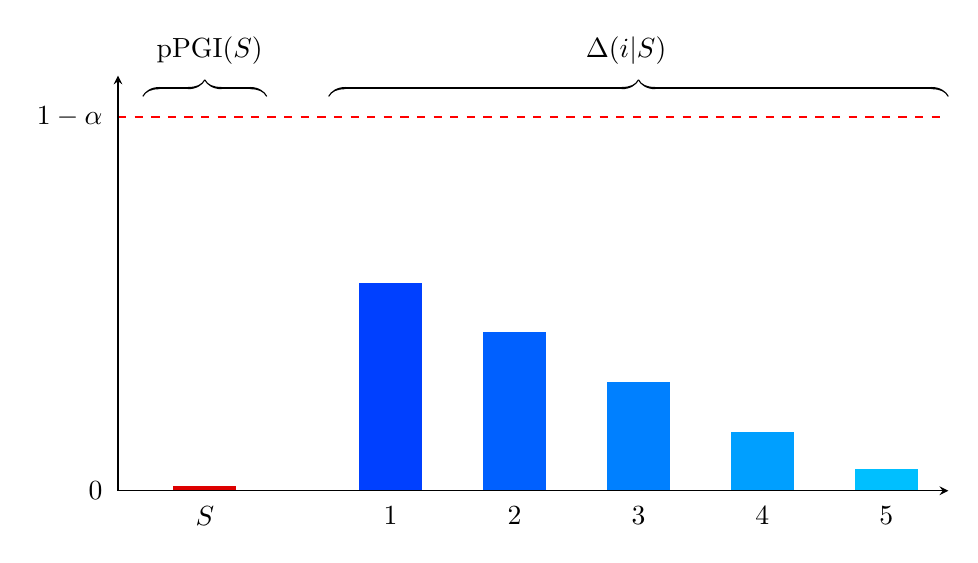
\begin{tikzpicture}
\begin{axis}[axis lines = left,
    /pgf/number format/1000 sep={},
    width=300,
    height=150,
    scale only axis,
    clip=false,
    separate axis lines,
    axis on top,
    xmin=0.3,
    xmax=7,
    xtick={1,2.5,3.5,4.5,5.5,6.5},
    x tick style={draw=none},
    xticklabels={$S$,1,2,3,4,5},
    ytick={0,0.9},
    y tick style={draw=none},
    yticklabels={0,$1-\alpha$},
    ymin=0,
    ymax=1,
    ]
    \addplot[s1,ybar,bar width=.5, fill]coordinates {(1,0.01)};
    \addplot[s2,ybar,bar width=.5, fill]coordinates{(2.5,0.5)};
    \addplot[s3,ybar,bar width=.5, fill]coordinates{(3.5,0.38)};
    \addplot[s4,ybar,bar width=.5, fill]coordinates{(4.5,0.26)};
    \addplot[s5,ybar,bar width=.5, fill]coordinates{(5.5,0.14)};
    \addplot[s6,ybar,bar width=.5, fill]coordinates{(6.5,0.05)};
    \addplot[dashed,red,thick] (0.3,0.9) -- (7,0.9);
    \node[anchor=center] at (1.04,1.06) {pPGI$(S)$};
    \node[anchor=center] at (4.4, 1.06) {$\Delta(i|S)$};
    \begin{scope}[decoration={calligraphic brace, amplitude=6pt}]
        \draw[thick, decorate] (2,0.95) -- (7,0.95);
        \draw[thick, decorate] (0.5,0.95) -- (1.5,0.95);
    \end{scope}
\end{axis}
\end{tikzpicture}
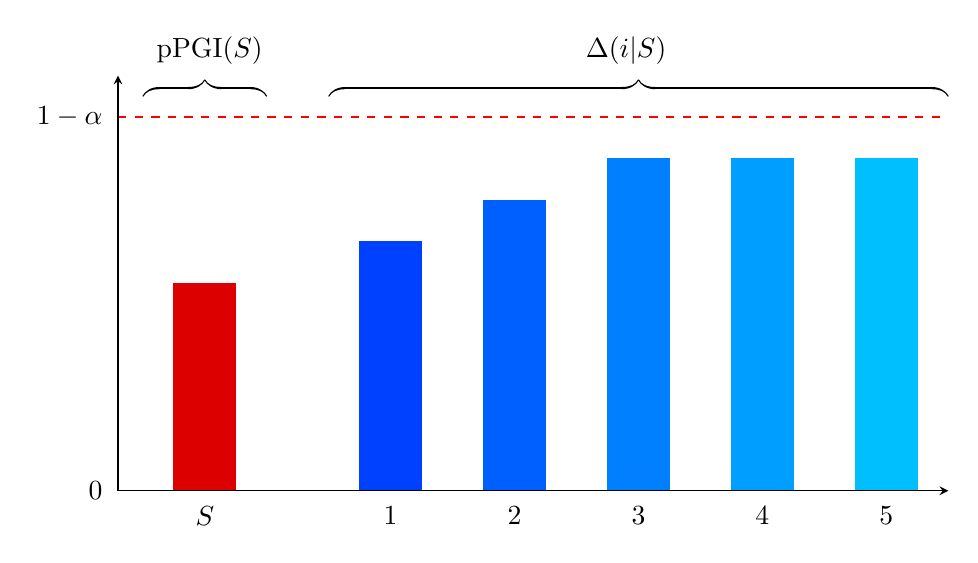
\begin{tikzpicture}
    \begin{axis}[axis lines = left,
        /pgf/number format/1000 sep={},
        width=300,
        height=150,
        scale only axis,
        clip=false,
        separate axis lines,
        axis on top,
        xmin=0.3,
        xmax=7,
        xtick={1,2.5,3.5,4.5,5.5,6.5},
        x tick style={draw=none},
        xticklabels={$S$,1,2,3,4,5},
        ytick={0,0.9},
        y tick style={draw=none},
        yticklabels={0,$1-\alpha$},
        ymin=0,
        ymax=1,
        ]
        \addplot[s1,ybar,bar width=.5, fill]coordinates {(1,0.5)};
        \addplot[s2,ybar,bar width=.5, fill]coordinates{(2.5,0.6)};
        \addplot[s3,ybar,bar width=.5, fill]coordinates{(3.5,0.7)};
        \addplot[s4,ybar,bar width=.5, fill]coordinates{(4.5,0.8)};
        \addplot[s5,ybar,bar width=.5, fill]coordinates{(5.5,0.8)};
        \addplot[s6,ybar,bar width=.5, fill]coordinates{(6.5,0.8)};
        
        \addplot[dashed,red,thick] (0.3,0.9) -- (7,0.9);
        \node[anchor=center] at (1.04,1.06) {pPGI$(S)$};
        \node[anchor=center] at (4.4, 1.06) {$\Delta(i|S)$};
        \begin{scope}[decoration={calligraphic brace, amplitude=6pt}]
            \draw[thick, decorate] (2,0.95) -- (7,0.95);
            \draw[thick, decorate] (0.5,0.95) -- (1.5,0.95);
        \end{scope}
    \end{axis}
\end{tikzpicture}
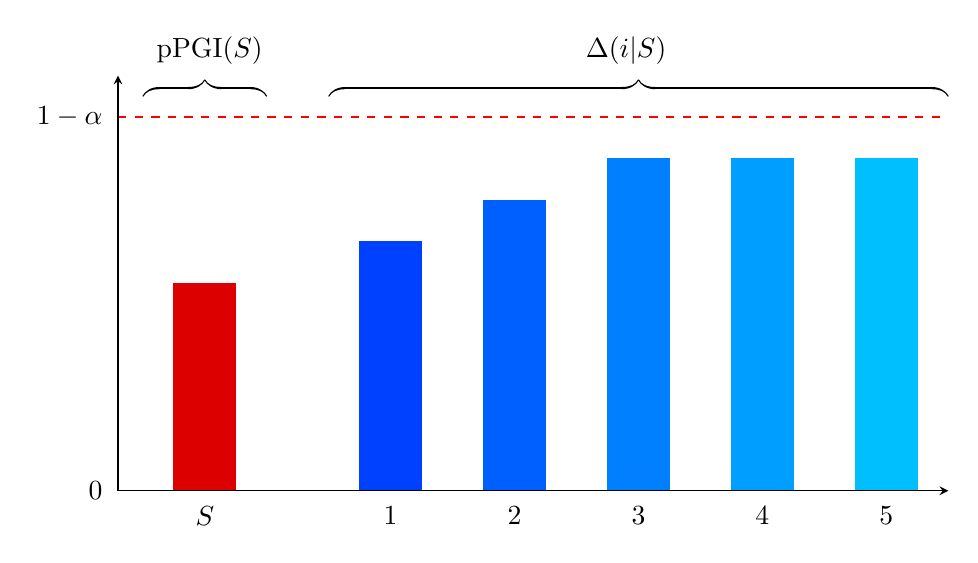
\begin{tikzpicture}
    \begin{axis}[axis lines = left,
        /pgf/number format/1000 sep={},
        width=300,
        height=150,
        scale only axis,
        clip=false,
        separate axis lines,
        axis on top,
        xmin=0.3,
        xmax=7,
        xtick={1,2.5,3.5,4.5,5.5,6.5},
        x tick style={draw=none},
        xticklabels={$S$,1,2,3,4,5},
        ytick={0,0.9},
        y tick style={draw=none},
        yticklabels={0,$1-\alpha$},
        ymin=0,
        ymax=1,
        ]
        \addplot[s1,ybar,bar width=.5, fill]coordinates {(1,0.5)};
        \addplot[s2,ybar,bar width=.5, fill]coordinates{(2.5,0.6)};
        \addplot[s3,ybar,bar width=.5, fill]coordinates{(3.5,0.7)};
        \addplot[s4,ybar,bar width=.5, fill]coordinates{(4.5,0.8)};
        \addplot[s5,ybar,bar width=.5, fill]coordinates{(5.5,0.8)};
        \addplot[s6,ybar,bar width=.5, fill]coordinates{(6.5,0.8)};
        \addplot[dashed,red,thick] (0.3,0.9) -- (7,0.9);
        \node[anchor=center] at (1.04,1.06) {pPGI$(S)$};
        \node[anchor=center] at (4.4, 1.06) {$\Delta(i|S)$};
        \begin{scope}[decoration={calligraphic brace, amplitude=6pt}]
            \draw[thick, decorate] (2,0.95) -- (7,0.95);
            \draw[thick, decorate] (0.5,0.95) -- (1.5,0.95);
        \end{scope}
    \end{axis}
\end{tikzpicture}


\end{document}